\chapter{Multilinear Functions (Tensors)}

A multivector multilinear function\footnote{We are following the treatment of Tensors in section 3--10 of \cite{H&S}.} is a 
multivector function $\f{T}{A_{1},\dots,A_{r}}$ that is linear in each of its arguments\footnote{We assume that the arguments 
are elements of a vector space or more generally a geometric algebra so that the concept of linearity is meaningful.} 
The tensor could be non-linearly dependent on a set of additional arguments such as the position coordinates $x^{i}$ in the 
case of a tensor field defined on a manifold.  If $x$ denotes the coordinate tuple for a manifold we denote the dependence 
of $T$ on $x$ by $\f{T}{A_{1},\dots,A_{r};x}$.
 
$T$ is a \emph{tensor} of degree $r$ if each variable $A_{j} \in \mathcal{V}_{n}$ ($\mathcal{V}_{n}$ is an 
$n$-dimensional vector space).  More generally if each 
$A_{j}\in\f{\mathcal{G}}{\mathcal{V}_{n}}$ (the geometric algebra of $\mathcal{V}_{n}$), we call $T$ an \emph{extensor} of
degree-$r$ on $\f{\mathcal{G}}{\mathcal{V}_{n}}$.

If the values of $\f{T}{a_{1},\dots,a_{r}}$ $\lp a_{j}\in\mathcal{V}_{n}\;\forall\; 1\le j \le r \rp$ are $s$-vectors 
(pure grade $s$ multivectors in 
$\f{\mathcal{G}}{\mathcal{V}_{n}}$) we say that $T$ has grade $s$ and rank $r+s$.  A tensor of grade zero is called a
\emph{multilinear form}.

In the normal definition of tensors as multilinear functions the tensor is defined as a multilinear mapping 
$$T:\bigtimes_{i=1}^{r}\mathcal{V}_{n}\rightarrow\Re,$$ so that the standard tensor definition is an example of a grade zero
degree/rank $r$ tensor in our definition.

\section{Algebraic Operations}
The properties of tensors are ($\alpha\in\Re$, $a_{j},b\in\mathcal{V}_{n}$, $T$ and $S$ are tensors of rank $r$,
and $\circ$ is any multivector multiplicative operation)
\begin{align}
	\f{T}{a_{1},\dots,\alpha a_{j},\dots,a_{r}} =& \alpha\f{T}{a_{1},\dots,a_{j},\dots,a_{r}}, \\
	\f{T}{a_{1},\dots,a_{j}+b,\dots,a_{r}} =& \f{T}{a_{1},\dots,a_{j},\dots,a_{r}}+ \f{T}{a_{1},\dots,a_{j-1},b,a_{j+1},\dots,a_{r}}, \\
	\f{\lp T\pm S\rp}{a_{1},\dots,a_{r}} \equiv& \f{T}{a_{1},\dots,a_{r}}\pm\f{S}{a_{1},\dots,a_{r}}.
\end{align}
Now let $T$ be of rank $r$ and $S$ of rank $s$ then the product of the two tensors is
\be
	\f{\lp T\circ S\rp}{a_{1},\dots,a_{r+s}} \equiv \f{T}{a_{1},\dots,a_{r}}\circ\f{S}{a_{r+1},\dots,a_{r+s}},
\ee
where ``$\circ$'' is any multivector multiplicative operation.

\section{Covariant, Contravariant, and Mixed Representations}

The arguments (vectors) of the multilinear fuction can be represented in terms of the basis vectors or the reciprocal basis vectors\footnote{When the $a_{j}$ vectors are expanded in terms of a basis we need a notatation that lets one determine which vector argument, $j$, the scalar components are associated with.  Thus when we expand the vector in terms of the basis we write
$a_{j} = a^{i_{j}}\eb_{i_{j}}$ with the Einstein summation convention applied over the $i_{j}$ indices. In the expansion the
$j$ in the $a^{i_{j}}$ determines which argument in the tensor function the $a^{i_{j}}$ coefficients are associated with.  Thus
it is always the subscript of the component super or subscript that determines the argument the coefficient is associated with.}
\begin{align}
	a_{j} =& a^{i_{j}}\eb_{i_{j}}, \label{vrep}\\
	      =& a_{i_{j}}\eb^{i_{j}}. \label{rvrep}
\end{align}
Equation~(\ref{vrep}) gives $a_{j}$ in terms of the basis vectors and eq~(\ref{rvrep}) in terms of the reciprocal basis vectors. The index
$j$ refers to the argument slot and the indices $i_{j}$ the components of the vector in terms of the basis.  The Einstein summation
convention is used throughout.  The covariant representation of the tensor is defined by
\begin{align}
	T\indices{_{i_{1}\dots i_{r}}} \equiv& \f{T}{\eb_{i_{1}},\dots,\eb_{i_{r}}} \\
	\f{T}{a_{1},\dots,a_{r}} =& \f{T}{a^{i_{1}}\eb_{i_{1}},\dots,a^{i_{r}}\eb_{i_{r}}} \nonumber \\
	                         =& \f{T}{\eb_{i_{1}},\dots,\eb_{i_{r}}}a^{i_{1}}\dots a^{i_{r}} \nonumber \\
	                         =& T\indices{_{i_{1}\dots i_{r}}}a^{i_{1}}\dots a^{i_{r}}.
\end{align}
Likewise for the contravariant representation
\begin{align}
	T\indices{^{i_{1}\dots i_{r}}} \equiv& \f{T}{\eb^{i_{1}},\dots,\eb^{i_{r}}} \\
	\f{T}{a_{1},\dots,a_{r}} =& \f{T}{a_{i_{1}}\eb^{i_{1}},\dots,a_{i_{r}}\eb^{i_{r}}} \nonumber \\
	                         =& \f{T}{\eb^{i_{1}},\dots,\eb^{i_{r}}}a_{i_{1}}\dots a_{i_{r}} \nonumber \\
	                         =& T\indices{^{i_{1}\dots i_{r}}}a_{i_{1}}\dots a_{i_{r}}.
\end{align}
One could also have a mixed representation
\begin{align}
	T\indices{_{i_{1}\dots i_{s}}^{i_{s+1}\dots i_{r}}} \equiv& \f{T}{\eb_{i_{1}},\dots,\eb_{i_{s}},\eb^{i_{s+1}}\dots\eb^{i_{r}}} \\
	\f{T}{a_{1},\dots,a_{r}} =& \f{T}{a^{i_{1}}\eb_{i_{1}},\dots,a^{i_{s}}\eb_{i_{s}},
	                            a_{i_{s+1}}\eb^{i_{s}},\dots,a_{i_{r}}\eb^{i_{r}}} \nonumber \\
	                         =& \f{T}{\eb_{i_{1}},\dots,\eb_{i_{s}},\eb^{i_{s+1}},\dots,\eb^{i_{r}}}
	                            a^{i_{1}}\dots a^{i_{s}}a_{i_{s+1}}\dots a_{i_{r}} \nonumber \\
	                         =& T\indices{_{i_{1}\dots i_{s}}^{i_{s+1}\dots i_{r}}}a^{i_{1}}\dots a^{i_{s}}a_{i_{s+1}},\dots a_{i_{r}}.
\end{align}
In the representation of $T$ one could have any combination of covariant (lower) and contravariant (upper) indices.

To convert a covariant index to a contravariant index simply consider
\begin{align}
	\f{T}{\eb_{i_{1}},\dots,\eb^{i_{j}},\dots,\eb_{i_{r}}} =& \f{T}{\eb_{i_{1}},\dots,g^{i_{j}k_{j}}\eb_{k_{j}},\dots,\eb_{i_{r}}} \nonumber \\
	                                                       =& g^{i_{j}k_{j}}\f{T}{\eb_{i_{1}},\dots,\eb_{k_{j}},\dots,\eb_{i_{r}}} \nonumber \\
	T\indices{_{i_{1}\dots}^{i_{j}}_{\dots i_{r}}} =& g^{i_{j}k_{j}}T\indices{_{i_{1}\dots i_{j}\dots i_{r}}}.
\end{align}
Similarly one could raise a lower index with $g_{i_{j}k_{j}}$.

\section{Contraction}
The contraction of a tensor between the $j^{th}$ and $k^{th}$ variables (slots) is\footnote{The notation of the l.h.s. of 
eq~(\ref{eq7_14a}) is new and is defined by $\nabla_{a_{k}} = \eb^{l_{k}}\partial_{a^{l_{k}}}$ and (the assumption of the
notation is that the $\partial_{a^{l_{k}}}$ can be factored out of the argument like a simple scalar)
\begin{align*}
	\f{T}{a_{i},\dots,a_{j-1},\nabla_{a_{k}},a_{j+1},\dots,a_{r}} \equiv& 
		\f{T}{a_{i},\dots,a_{j-1},\eb^{l_{k}}\partial_{a^{l_{k}}},a_{j+1},\dots,a^{i_{k}}\eb_{i_{k}},\dots,a_{r}} \\
	=& \f{T}{a_{i},\dots,a_{j-1},\eb_{j_{k}}g^{j_{k}l_{k}}\partial_{a^{l_{k}}},a_{j+1},\dots,a^{i_{k}}\eb_{i_{k}},\dots,a_{r}} \\
	=& g^{j_{k}l_{k}}\partial_{a^{l_{k}}}a^{i_{k}}\f{T}{a_{i},\dots,a_{j-1},\eb_{j_{k}},a_{j+1},\dots,\eb_{i_{k}},\dots,a_{r}} \\
	=& g^{j_{k}l_{k}}\delta_{l_{k}}^{i_{k}}\f{T}{a_{i},\dots,a_{j-1},\eb_{j_{k}},a_{j+1},\dots,\eb_{i_{k}},\dots,a_{r}} \\
	=& g^{j_{k}i_{k}}\f{T}{a_{i},\dots,a_{j-1},\eb_{j_{k}},a_{j+1},\dots,\eb_{i_{k}},\dots,a_{r}} \\
	=& g^{j_{k}i_{k}}T_{i_{1}\dots i_{j-1}j_{k}i_{j+1}\dots i_{k}\dots i_{r}}
		a^{i_{1}}\dots\breve{a}^{i_{j}}\dots\breve{a}^{i_{k}}\dots a^{i_{r}}.
\end{align*}}
\be
	\f{T}{a_{i},\dots,a_{j-1},\nabla_{a_{k}},a_{j+1},\dots,a_{r}} = \nabla_{a_{j}}\cdot\lp\nabla_{a_{k}}\f{T}{a_{1},\dots,a_{r}}\rp.\label{eq7_14a}
\ee
This operation reduces the rank of the tensor by two.  This definition gives the standard results for \emph{metric contraction} which is
proved as follows for a rank $r$ grade zero tensor (the circumflex ``$\breve{\:\:}$'' indicates that a term is to be deleted from the product).
\begin{align}
	\f{T}{a_{1},\dots,a_{r}} =& a^{i_{1}}\dots a^{i_{r}}T_{i_{1}\dots i_{r}} \\
	\nabla_{a_{j}}T =& \eb^{l_{j}} a^{i_{1}}\dots\lp\partial_{a^{l_j}}a^{i_{j}}\rp\dots a_{i_{r}}T_{i_{1}\dots i_{r}} \nonumber \\
	=& \eb^{l_{j}}\delta_{l_{j}}^{i_{j}} a^{i_{1}}\dots \breve{a}^{i_{j}}\dots a^{i_{r}}T_{i_{1}\dots i_{r}} \\
	\nabla_{a_{m}}\cdot\lp\nabla_{a_{j}}T\rp =& \eb^{k_{m}}\cdot\eb^{l_{j}}\delta_{l_{j}}^{i_{j}} 
	                                          a^{i_{1}}\dots \breve{a}^{i_{j}}\dots\lp\partial_{a^{k_m}}a^{i_{m}}\rp 
	                                          \dots a^{i_{r}}T_{i_{1}\dots i_{r}} \nonumber \\
	                                         =& g^{k_{m}l_{j}}\delta_{l_{j}}^{i_{j}}\delta_{k_{m}}^{i_{m}} 
	                                          a^{i_{1}}\dots \breve{a}^{i_{j}}\dots\breve{a}^{i_{m}} 
	                                          \dots a^{i_{r}}T_{i_{1}\dots i_{r}} \nonumber \\
	                                         =& g^{i_{m}i_{j}}a^{i_{1}}\dots \breve{a}^{i_{j}}\dots\breve{a}^{i_{m}} 
	                                          \dots a^{i_{r}}T_{i_{1}\dots i_{j}\dots i_{m}\dots i_{r}} \nonumber \\
	                                         =& g^{i_{j}i_{m}}a^{i_{1}}\dots \breve{a}^{i_{j}}\dots\breve{a}^{i_{m}} 
	                                          \dots a^{i_{r}}T_{i_{1}\dots i_{j}\dots i_{m}\dots i_{r}}  \nonumber \\
	                                         =& \lp g^{i_{j}i_{m}}T_{i_{1}\dots i_{j}\dots i_{m}\dots i_{r}}\rp a^{i_{1}}\dots
	                                          \breve{a}^{i_{j}}\dots\breve{a}^{i_{m}}\dots a^{i_{r}} \label{eq108}
\end{align} 
Equation~(\ref{eq108}) is the correct formula for the metric contraction of a tensor.

If we have a mixed representation of a tensor, $T\indices{_{i_{1}\dots}^{i_{j}}_{\dots i_{k}\dots i_{r}}}$, 
and wish to contract between an upper and lower index ($i_{j}$ and $i_{k}$) first lower the upper index and then use eq~(\ref{eq108})
to contract the result.  Remember lowering the index does \emph{not} change the tensor, only the \emph{representation} of the tensor,
while contraction results in a \emph{new} tensor.  First lower index
\be
	T\indices{_{i_{1}\dots}^{i_{j}}_{\dots i_{k}\dots i_{r}}} \xRightarrow{\mbox{\tiny Lower Index}} g_{i_{j}k_{j}}T\indices{_{i_{1}\dots}^{k_{j}}_{\dots i_{k}\dots i_{r}}}	
\ee
Now contract between $i_{j}$ and $i_{k}$ and use the properties of the metric tensor.
\begin{align}
	g_{i_{j}k_{j}}T\indices{_{i_{1}\dots}^{k_{j}}_{\dots i_{k}\dots i_{r}}} \xRightarrow{\mbox{\tiny Contract}}&
				g^{i_{j}i_{k}}g_{i_{j}k_{j}}T\indices{_{i_{1}\dots}^{k_{j}}_{\dots i_{k}\dots i_{r}}} \nonumber \\
				=& \delta_{k_{j}}^{i_{k}}T\indices{_{i_{1}\dots}^{k_{j}}_{\dots i_{k}\dots i_{r}}}. \label{114a}
\end{align}
Equation~(\ref{114a}) is the standard formula for contraction between upper and lower indices of a mixed tensor.

\section{Differentiation}
If $\f{T}{a_{1},\dots,a_{r};x}$ is a tensor field (a function of the position vector, $x$, for a vector space or the coordinate
tuple, $x$, for a manifold) the tensor directional derivative is defined as
\begin{align}
	\mathcal{D}\f{T}{a_{1},\dots,a_{r};x} \equiv \lp a_{r+1}\cdot\nabla\rp\f{T}{a_{1},\dots,a_{r};x},
\end{align}
assuming the $a^{i_{j}}$ coefficients are not a function of the coordinates.

This gives for a grade zero rank $r$ tensor
\begin{align}
	\lp a_{r+1}\cdot\nabla\rp\f{T}{a_{1},\dots,a_{r}} =& a^{i_{r+1}}\partial_{x^{i_{r+1}}}a^{i_{1}}\dots a^{i_{r}}
													    T_{i_{1}\dots i_{r}}, \nonumber \\
													 =& a^{i_{1}}\dots a^{i_{r}}a^{i_{r+1}}
													    \partial_{x^{i_{r+1}}}T_{i_{1}\dots i_{r}}. 
\end{align}

\section{From Vector/Multivector to Tensor}

A rank one tensor corresponds to a vector since it satisfies all the axioms for a vector space, but a vector in not necessarily a tensor since not all vectors
are multilinear (actually in the case of vectors a linear function) functions.  However, there is a simple isomorphism between vectors and 
rank one tensors defined by the mapping $\f{v}{a}:\mathcal{V}\rightarrow\Re$ such that if $v,a \in\mathcal{V}$
\be
	\f{v}{a} \equiv v\cdot a.
\ee
So that if $v = v^{i}\eb_{i} = v_{i}\eb^{i}$ the covariant and contravariant representations of $v$ are 
(using $\eb^{i}\cdot\eb_{j} = \delta^{i}_{j}$)
\be
	\f{v}{a} = v_{i}a^{i} = v^{i}a_{i}.
\ee
The equivalent mapping from a pure $r$-grade multivector $A$ to a rank-$r$ tensor $\f{A}{a_{1},\dots,a_{r}}$ is
\be
	\f{A}{a_{1},\dots,a_{r}} = A\cdot\paren{a_{1}\W\dots\W a_{r}}.\label{eq7_24a}
\ee
Note that since the sum of two tensor of different ranks is not defined we cannot represent a spinor with tensors.  
Additionally, even if we allowed for the summation of tensors of different ranks we would also have to redefine the
tensor product to have the properties of the geometric wedge product.  Likewise, multivectors can only represent 
completely antisymmetric tensors of rank less than or equal to the dimension of the base vector space. 

\section{Parallel Transport Definition and Example}
The defintion of parallel transport is that if $a$ and $b$ are tangent vectors in the tangent spaced of the manifold then
\be
	\paren{a\cdot\nabla_{x}}b = 0 \label{eq108a}
\ee
if $b$ is parallel transported in the direction of a (infinitesimal parallel transport).  Since $b = b^{i}\eb_{i}$ and the derivatives of $\eb_{i}$ are functions of the $x^{i}$'s then the $b^{i}$'s are
also functions of the $x^{i}$'s so that in order for eq~(\ref{eq108a}) to be satisfied we have
\begin{align}
	\paren{a\cdot\nabla_{x}}b =& a^{i}\partial_{x^{i}}\paren{b^{j}\eb_{j}} \nonumber \\
	                          =& a^{i}\paren{\paren{\partial_{x^{i}}b^{j}}\eb_{j} + b^{j}\partial_{x^{i}}\eb_{j}} \nonumber \\
	                          =& a^{i}\paren{\paren{\partial_{x^{i}}b^{j}}\eb_{j} + b^{j}\Gamma_{ij}^{k}\eb_{k}} \nonumber \\
	                          =& a^{i}\paren{\paren{\partial_{x^{i}}b^{j}}\eb_{j} + b^{k}\Gamma_{ik}^{j}\eb_{j}}\nonumber \\
	                          =& a^{i}\paren{\paren{\partial_{x^{i}}b^{j}} + b^{k}\Gamma_{ik}^{j}}\eb_{j} = 0.
\end{align}
Thus for $b$ to be parallel transported (infinitesimal parallel transport in any direction $a$) we must have
\be
	\partial_{x^{i}}b^{j} = -b^{k}\Gamma_{ik}^{j}. \label{eq121a}
\ee
The geometric meaning of parallel transport is that for an infinitesimal rotation and dilation of the basis vectors (cause by infinitesimal changes in the $x^{i}$'s) the direction and magnitude of the vector $b$ does not change to first order.

If we apply eq~(\ref{eq121a}) along a parametric curve defined by $\f{x^{j}}{s}$ we have
\begin{align}
	\deriv{b^{j}}{s}{} =& \deriv{x^{i}}{s}{}\pdiff{b^{j}}{x^{i}} \nonumber \\
	                   =& -b^{k}\deriv{x^{i}}{s}{}\Gamma_{ik}^{j}, \label{eq122a}
\end{align}
and if we define the initial conditions $\f{b^{j}}{0}\eb_{j}$.  Then eq~(\ref{eq122a}) is a system of first order
linear differential equations with intial conditions and the solution, $\f{b^{j}}{s}\eb_{j}$, is the parallel transport of the
vector $\f{b^{j}}{0}\eb_{j}$.

An equivalent formulation for the parallel transport equation is to let $\f{\gamma}{s}$ be a parametric curve in the manifold
defined by the tuple $\f{\gamma}{s} = \paren{\f{x^{1}}{s},\dots,\f{x^{n}}{s}}$.  Then the tangent to $\f{\gamma}{s}$ is given by
\be
	\deriv{\gamma}{s}{} \equiv \deriv{x^{i}}{s}{}\eb_{i}
\ee
and if $\f{v}{x}$ is a vector field on the manifold then
\begin{align}
	\paren{\deriv{\gamma}{s}{}\cdot\nabla_{x}}v =& \deriv{x^{i}}{s}{}\pdiff{}{x^{i}}\paren{v^{j}\eb_{j}} \nonumber \\
	     =&\deriv{x^{i}}{s}{}\paren{\pdiff{v^{j}}{x^{i}}\eb_{j}+v^{j}\pdiff{\eb_{j}}{x^{i}}} \nonumber \\
	     =&\deriv{x^{i}}{s}{}\paren{\pdiff{v^{j}}{x^{i}}\eb_{j}+v^{j}\Gamma^{k}_{ij}\eb_{k}} \nonumber \\
	     =&\deriv{x^{i}}{s}{}\pdiff{v^{j}}{x^{i}}\eb_{j}+\deriv{x^{i}}{s}{}v^{k}\Gamma^{j}_{ik}\eb_{j} \nonumber \\
	     =&\paren{\deriv{v^{j}}{s}{}+\deriv{x^{i}}{s}{}v^{k}\Gamma^{j}_{ik}}\eb_{j} \nonumber \\
	     =& 0. \label{eq124a}
\end{align}
Thus eq~(\ref{eq124a}) is equivalent to eq~(\ref{eq122a}) and parallel transport of a vector field along a curve is 
equivalent to the directional derivative of the vector field in the direction of the tangent to the curve being zero.  

As a specific example of parallel transport consider a spherical manifold with a series of concentric circular curves and
paralle transport a vector along each curve.  Note that the circular curves are defined by 
\begin{align*}
	\f{u}{s} =& u_{0}+a\:\f{\cos}{\bfrac{s}{2\pi a}} \\
	\f{v}{s} =& v_{0}+a\:\f{\sin}{\bfrac{s}{2\pi a}} 
\end{align*}
where $u$ and $v$ are the manifold coordinates. The spherical manifold is defined by
\begin{align*}
	x =& \f{\cos}{u}\f{cos}{v} \\
	y =& \f{\cos}{u}\f{sin}{v} \\
	z =& \f{\sin}{u}. 
\end{align*}
Note that due to the dependence of the metric on the coordinates circles do not necessarily appear to be circular in the plots
depending on the values of $u_{0}$ and $v_{0}$ (see fig~\ref{fig2}). For symmetrical circles we have fig~\ref{fig1} 
and for asymmetrical circles we have fig~\ref{fig2}.  Note that the appearance of the transported (black) vectors is an optical
illusion due to the projection.  If the sphere were rotated we would see that the transported vectors are in the tangent 
space of the manifold.
\begin{figure}[h]
	\begin{center}
	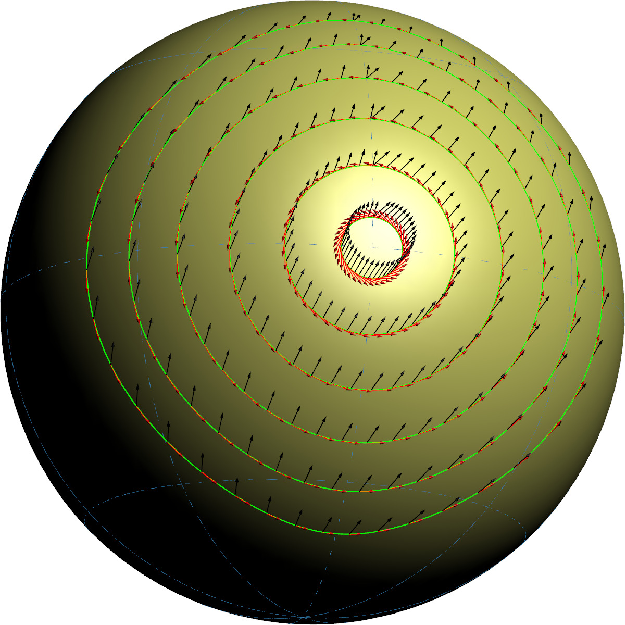
\includegraphics[scale=1]{parallel_transport1} 
	\end{center}
	\caption{Parallel transport for $u_{0}=0$ and $v_{0}=0$. Red vectors are tangents to circular curves and black vectors
	are the vectors being transported.}\label{fig1}
\end{figure}
\begin{figure}[h]
	\begin{center}
	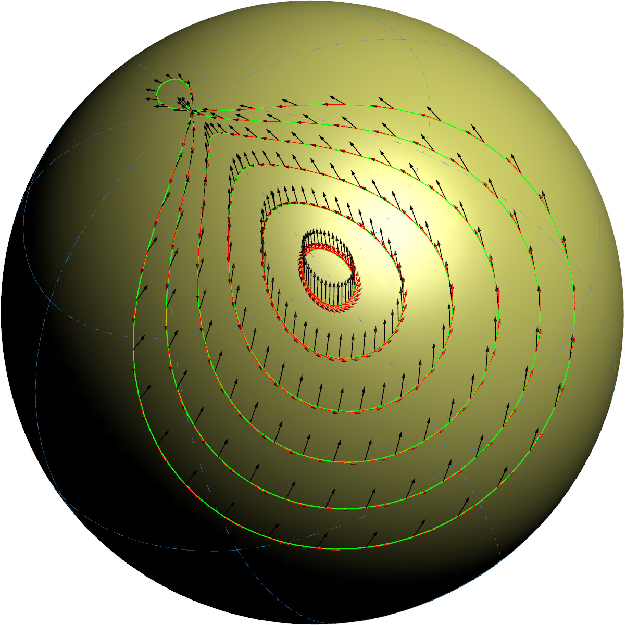
\includegraphics[scale=1]{parallel_transport2} 
	\end{center}
	\caption{Parallel transport for $u_{0}=\pi/4$ and $v_{0}=\pi/4$. Red vectors are tangents to circular curves and black vectors
	are the vectors being transported.}\label{fig2}
\end{figure}

If $\f{\gamma}{s} = \paren{\f{u}{s},\f{v}{s}}$ defines the transport curve then
\be
	\deriv{\gamma}{s}{} = \deriv{u}{s}{}\eb_{u}+\deriv{v}{s}{}\eb_{v}
\ee
and the transport equations are
\begin{align}
	\paren{\deriv{\gamma}{s}{}\cdot\nabla} f =& \paren{\deriv{u}{s}{}\pdiff{f^{u}}{u}+\deriv{v}{s}{}\pdiff{f^{u}}{v}
	                                            -\f{\sin}{u}\f{\cos}{u}\deriv{v}{s}{}f^{v}}\eb_{u}+\nonumber \\
	                                          & \paren{\deriv{u}{s}{}\pdiff{f^{v}}{u}+\deriv{v}{s}{}\pdiff{f^{v}}{v}
	                                            +\bfrac{\f{\cos}{u}}{\f{\sin}{u}}
	                                             \paren{\deriv{u}{s}{}f^{v}+\deriv{v}{s}{}f^{u}}}\eb_{u}  \nonumber \\
	                                         =& \paren{\deriv{f^{u}}{s}{}
	                                            -\f{\sin}{u}\f{\cos}{u}\deriv{v}{s}{}f^{v}}\eb_{u}+\nonumber \\
	                                          & \paren{\deriv{f^{v}}{s}{}
	                                            +\bfrac{\f{\cos}{u}}{\f{\sin}{u}}
	                                             \paren{\deriv{u}{s}{}f^{v}+\deriv{v}{s}{}f^{u}}}\eb_{u}  = 0  \\
	 \deriv{f^{u}}{s}{} =& \;\f{\sin}{u}\f{\cos}{u}\deriv{v}{s}{}f^{v} \\
	 \deriv{f^{v}}{s}{} =& \;-\bfrac{\f{\cos}{u}}{\f{\sin}{u}}
	                                             \paren{\deriv{u}{s}{}f^{v}+\deriv{v}{s}{}f^{u}}
\end{align}
If the tensor component representation is contra-variant (superscripts instead of subscripts) we must use the covariant component representation of
the vector arguements of the tensor, $a = a_{i}\eb^{i}$.  Then the definition of parallel transport gives
\begin{align}
	\paren{a\cdot\nabla_{x}}b =& a^{i}\partial_{x^{i}}\paren{b_{j}\eb^{j}} \nonumber \\
	                          =& a^{i}\paren{\paren{\partial_{x^{i}}b_{j}}\eb^{j} + b_{j}\partial_{x^{i}}\eb^{j}},
\end{align}
and we need
\be
	\paren{\partial_{x^{i}}b_{j}}\eb^{j} + b_{j}\partial_{x^{i}}\eb^{j} = 0. \label{eq111a}
\ee
To satisfy equation~(\ref{eq111a}) consider the following
\begin{align}
	\partial_{x^{i}}\paren{\eb^{j}\cdot\eb_{k}} =& 0 \nonumber \\
	\paren{\partial_{x^{i}}\eb^{j}}\cdot\eb_{k} + \eb^{j}\cdot\paren{\partial_{x^{i}}\eb_{k}} =& 0  \nonumber \\
	\paren{\partial_{x^{i}}\eb^{j}}\cdot\eb_{k} + \eb^{j}\cdot\eb_{l}\Gamma_{ik}^{l} =& 0 \nonumber \\
	\paren{\partial_{x^{i}}\eb^{j}}\cdot\eb_{k} + \delta_{l}^{j}\Gamma_{ik}^{l} =& 0 \nonumber \\
	\paren{\partial_{x^{i}}\eb^{j}}\cdot\eb_{k} + \Gamma_{ik}^{j} =& 0 \nonumber \\
	\paren{\partial_{x^{i}}\eb^{j}}\cdot\eb_{k} =& -\Gamma_{ik}^{j}
\end{align}
Now dot eq~(\ref{eq111a}) into $\eb_{k}$ giving\footnote{These equations also show that
\be
	\partial_{x^{i}}\eb^{j} = -\Gamma_{ik}^{j}\eb^{k}.
\ee}
\begin{align}
	\paren{\partial_{x^{i}}b_{j}}\eb^{j}\cdot\eb_{k} + b_{j}\paren{\partial_{x^{i}}\eb^{j}}\cdot\eb_{k} =& 0  \nonumber \\
	\paren{\partial_{x^{i}}b_{j}}\delta_{j}^{k} - b_{j}\Gamma_{ik}^{j} =& 0 \nonumber \\
	\paren{\partial_{x^{i}}b_{k}} = b_{j}\Gamma_{ik}^{j}.
\end{align}

\section{Covariant Derivative of Tensors}
The covariant derivative of a tensor field $\f{T}{a_{1},\dots,a_{r};x}$ ($x$ is the coordinate tuple of which $T$ can be a non-linear function) in the direction $a_{r+1}$ is (remember $a_{j} = a^{k_{j}}\eb_{k_{j}}$ and the $\eb_{k_{j}}$ can be functions of $x$)
the directional derivative of $\f{T}{a_{1},\dots,a_{r};x}$ where all the $a_{i}$ vector arguments of $T$ are parallel transported. 

Thus if we have a mixed representation of a tensor 
\be
\f{T}{a_{1},\dots,a_{r};x} = 
	\f{T\indices{_{i_{1}\dots i_{s}}^{i_{s+1}\dots i_{r}}}}{x}a^{i_{1}}\dots a^{i_{s}}a_{i_{s+1}}\dots a_{i_{r}},
\ee
the covariant derivative of the tensor is
\begin{align}
	\paren{a_{r+1}\cdot D} \f{T}{a_{1},\dots,a_{r};x} =& 
		\pdiff{T\indices{_{i_{1}\dots i_{s}}^{i_{s+1}\dots i_{r}}}}{x^{r+1}}a^{i_{1}}\dots a^{i_{s}}a_{i_{s+1}}\dots a_{i_{r}}
		a^{i_{r+1}} \nonumber \\
		&\hspace{-0.5in}+ \sum_{p=1}^{s}\pdiff{a^{i_{p}}}{x^{i_{r+1}}}T\indices{_{i_{1}\dots i_{s}}^{i_{s+1}\dots i_{r}}}a^{i_{1}}\dots
		\breve{a}^{i_{p}}\dots a^{i_{s}}a_{i_{s+1}}\dots a_{i_{r}}a^{i_{r+1}} \nonumber \\
		&\hspace{-0.5in}+ \sum_{q=s+1}^{r}\pdiff{a_{i_{p}}}{x^{i_{r+1}}}T\indices{_{i_{1}\dots i_{s}}^{i_{s+1}\dots i_{r}}}a^{i_{1}}\dots
		a^{i_{s}}a_{i_{s+1}}\dots\breve{a}_{i_{q}}\dots a_{i_{r}}a^{i_{r+1}} \nonumber \\
		=& \pdiff{T\indices{_{i_{1}\dots i_{s}}^{i_{s+1}\dots i_{r}}}}{x^{r+1}}a^{i_{1}}\dots a^{i_{s}}a_{i_{s+1}}\dots a^{r}_{i_{r}}
		a^{i_{r+1}} \nonumber \\
		&\hspace{-0.5in}- \sum_{p=1}^{s}\Gamma_{i_{r+1}l_{p}}^{i_{p}}T\indices{_{i_{1}\dots i_{p}\dots i_{s}}^{i_{s+1}
		\dots i_{r}}}a^{i_{1}}\dots
		a^{l_{p}}\dots a^{i_{s}}a_{i_{s+1}}\dots a_{i_{r}}a^{i_{r+1}} \nonumber \\
		&\hspace{-0.5in}+ \sum_{q=s+1}^{r}\Gamma_{i_{r+1}i_{q}}^{l_{q}}T\indices{_{i_{1}\dots i_{s}}^{i_{s+1}\dots i_{q}
		\dots i_{r}}}a^{i_{1}}\dots
		a^{i_{s}}a_{i_{s+1}}\dots a_{l_{q}}\dots a_{i_{r}}a^{i_{r+1}}	.	\label{eq126a}
\end{align}
From eq~(\ref{eq126a}) we obtain the components of the covariant derivative to be
\begin{align}
	\pdiff{T\indices{_{i_{1}\dots i_{s}}^{i_{s+1}\dots i_{r}}}}{x^{r+1}}
	- \sum_{p=1}^{s}\Gamma_{i_{r+1}l_{p}}^{i_{p}}T\indices{_{i_{1}\dots i_{p}\dots i_{s}}^{i_{s+1}\dots i_{r}}}
	+ \sum_{q=s+1}^{r}\Gamma_{i_{r+1}i_{q}}^{l_{q}}T\indices{_{i_{1}\dots i_{s}}^{i_{s+1}\dots i_{q}\dots i_{r}}}.
\end{align}
To extend the covariant derivative to tensors with multivector values in the tangent space (geometric algebra of the
tangent space) we start with the coordinate free definition of the covariant derivative of a conventional tensor using
the following notation.  Let $\f{T}{a_{1},\dots,a_{r};x}$ be a conventional tensor then the directional covariant 
derivative is
\be
	\paren{b\cdot D}T = a^{i_{1}}\dots a^{i_{r}}\paren{b\cdot\nabla}\f{T}{e_{i_{1}},\dots,e_{i_{r}};x}
						   -\sum_{j=1}^{r}\f{T}{a_{1},\dots,\paren{b\cdot\nabla}a_{j},\dots,a_{r};x}.	\label{eq137a}
\ee
The first term on the r.h.s. of eq~(\ref{eq137a}) is the directional derivative of $T$ if we assume that the component 
coefficients of each of the $a_{j}$ does not change if the coordinate tuple changes. The remaining terms in 
eq~(\ref{eq137a}) insure that for the totality of eq~(\ref{eq137a}) the directional derivative $\paren{b\cdot\nabla}T$
is the same as that when all the  $a_{j}$ vectors are parallel transported.  If in eq~(\ref{eq137a}) we let 
$b\cdot\nabla$ be the directional derivative for a multivector field we have generalized the definintion of covariant
derivative to include the cases where $\f{T}{a_{1},\dots,a_{r};x}$ is a multivector and not only a scalar.  Basically in 
eq~(\ref{eq137a}) the terms $\f{T}{e_{i_{1}},\dots,e_{i_{r}};x}$ are multivector fields and 
$\paren{b\cdot\nabla}\f{T}{e_{i_{1}},\dots,e_{i_{r}};x}$ is the direction derivative of each of the multivector fields that
make up the component representation of the multivector tensor.  The remaining terms in eq~(\ref{eq137a}) take into account
that for parallel transport of the $a_{i}$'s the coefficients $a^{i_{j}}$ are implicit functions of the coordinates
$x^{k}$. If we define the symbol $\nabla_{x}$ to only refer to taking the geometric derivative with respect to an explicit
dependence on the $x$ coordinate tuple we can recast eq~(\ref{eq137a}) into
\be
	\paren{b\cdot D}T = \paren{b\cdot\nabla_{x}}\f{T}{a_{1},\dots,a_{r};x}
						   -\sum_{j=1}^{r}\f{T}{a_{1},\dots,\paren{b\cdot\nabla}a_{j},\dots,a_{r};x}.	\label{eq137a}
\ee

\section{Coefficient Transformation Under Change of Variable}
In the previous sections on tensors a transformation of coordinate tuples 
$\f{\bar{x}}{x} = \paren{\f{\bar{x}^{i}}{x},\dots,\f{\bar{x}^{n}}{x}}$,
where $x=\paren{x^{1},\dots,x^{n}}$, is not mentioned since the definition of a tensor as a multilinear function is 
invariant to the representation of the vectors (coordinate system).  From our tensor definitions the effect of a coordinate
transformation on the tensor components is simply calculated.

If $\f{R}{x} = \f{R}{\bar{x}}$ is the defining vector function for a vector manifold ($R$ is in the embedding space of the
manifold) then\footnote{For an abstract manifold the equation $\bar{\eb}_{i} = \pdiff{x^{j}}{\bar{x}^{i}}\eb_{j}$ can be
used as an defining relationship.}
\begin{align}
	\eb_{i} =& \pdiff{R}{x^{i}} = \pdiff{\bar{x}^{j}}{x^{i}}\bar{\eb}_{j} \\
	\bar{\eb}_{i} =& \pdiff{R}{\bar{x}^{i}} =  \pdiff{x^{j}}{\bar{x}^{i}}\eb_{j}.
\end{align}
Thus we have
\begin{align}
	\f{T}{\eb_{i_{1}},\dots,\eb_{i_{1}}} =& T_{i_{1}\dots i_{r}} \\
	\f{T}{\bar{\eb}_{j_{1}},\dots,\bar{\eb}_{j_{1}}} =& \bar{T}_{j_{1}\dots j_{r}} \\
	\f{T}{\eb_{i_{1}},\dots,\eb_{i_{1}}} =& \f{T}{\pdiff{\bar{x}^{j_{1}}}{x^{i_{1}}}\bar{\eb}_{j_{1}},
	                                        \dots,\pdiff{\bar{x}^{j_{r}}}{x^{i_{r}}}\bar{\eb}_{j_{1}}} \\
	                                     =& \pdiff{\bar{x}^{j_{1}}}{x^{i_{1}}}\dots \pdiff{\bar{x}^{j_{r}}}{x^{i_{r}}}
	                                     \f{T}{\bar{\eb}_{j_{1}},\dots,\bar{\eb}_{j_{1}}} \\
	T_{i_{1}\dots i_{r}} =&  \pdiff{\bar{x}^{j_{1}}}{x^{i_{1}}}\dots\pdiff{\bar{x}^{j_{r}}}{x^{i_{r}}}
	                                     \bar{T}_{j_{1}\dots j{r}}. \label{eq7_51a} 
\end{align}
Equation~(\ref{eq7_51a}) is the standard formula for the transformation of tensor components.
